% Term project, 2011 Jan Pokorny <xpokor04@stud.fit.vutbr.cz>
%==============================================================================
\chapter{Rozhraní \texttt{code listener}}
\label{chap:code-listener}
%==============================================================================

Pokud se hovoří o rozhraní \texttt{code listener} \cite{web:FITVUTBR:VeriFIT:CodeListener},
má se výrazem \uv{rozhraní} na mysli především ten fakt, že jde softwarový
celek (přesněji knihovnu) zajišťující propojení dalších k tomu uzpůsobených
komponent. V užším pojetí \ndash\ a bude tomu tak i v dalším textu \ndash\ jde ovšem
za \uv{rozhraní} považovat skutečné rozhraní k této knihovně určené
příslušným hlavičkovým souborem \texttt{code\_listener.h}.

Knihovna tvoří infrastrukturu pro provádění analýz zdrojového kódu, kdy
propojuje komponenty provádějící extrakci syntaktických a sémantických
informací ze zdrojových kódů programů a komponenty obstarávající jejich
další vyhodnocení. Nejprve je knihovna stručně představena v obecnější rovině,
pak v rovině použití tohoto rozhraní.

\section{Knihovna základ infrastruktury pro statickou analýzu}

Samotné analýze kódu vždy předchází fáze předzpracování (tj. lexikální,
syntaktické/sémantické analýzy, dále jen shrnutu pojmem \uv{parsování})
zdrojových souborů do podoby nějaké vnitřní reprezentace, přes syntaktický
strom až po \emph{graf toku řízení} (\emph{control flow graph}, \emph{CFG}).
Tato příprava pracovních dat pro další usuzování nad nimi může být
poměrně komplexní (například u jazyka C se ho účastní také preprocesor),
ale naštěstí existují odladěné implementace nejen v rámci překladačů
daných jazyků, ale také v samostatných projektech typu \texttt{sparse}
(viz kap.\,\ref{chap:sparse}). Je tedy nasnadě použít prověřená řešení, ovšem
nemůžeme předpokládat nějaké jednotné rozhraní jejich výstupu.

Tento problém řeší právě knihovna \texttt{code listener}, kdy se pro každou
komponentu, kterou lze a je potřeba využít k parsování kódu, vytvoří
\emph{adaptér} (\emph{wrapper}) převádějící výstup této komponenty
do podoby vyžadované předmětným rozhraním, což zajistí unifikovaný
vstup pro komponenty dalšího zpracování. V současnosti v rámci širšího
projektu existuje a primárně se pro parsování používá adaptér integrovaný
jako zásuvný modul do překladače GCC a cílem diplomové práce
by pak mělo být obdobné využití (s pomocí vytvořeného adaptéru) nástroje
\texttt{sparse} pojednaného v kap.\,\ref{chap:sparse}.

Zatím byla diskutována pouze jedna strana propojovacího rozhraní, a sice
ta, která se také jinak označuje jako \emph{front-end}, poněvadž slouží
komponentám, jež přímo \uv{čelí} vstupním souborům s kódem programu
k analýze. Jeho reprezentace je pak skrze rozhraní unifikovaným způsobem
předána \uv{dozadu}, konkrétnímu \emph{back-endu} připojenému na opačné straně
tohoto rozhraní.

Mimo samotné rozhraní pro přenos reprezentace kódu je přítomna
také vrstva sloužící jako uložiště. Celý popsaný koncept ilustruje
blokové schéma na obr.\,\ref{fig:code-listener:api}.

\hspace*{\fill}\\[-\baselineskip]
\begin{figure}[!h]
    \begin{center}
        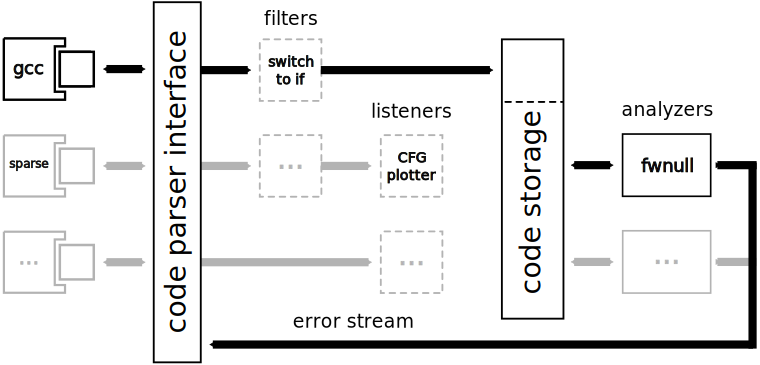
\includegraphics[width=1\textwidth,keepaspectratio]{fig/cl-block-diagram}
        \label{fig:code-listener:api}
        \caption{Blokové schéma rozhraní pro analýzu zdrojového kódu
                 \texttt{code listener} (převzato z \cite{web:FITVUTBR:VeriFIT:CodeListener})}
    \end{center}
\end{figure}


\section{Implementační stránka rozhraní}

Rozhraní \texttt{code listener} je dáno definicí typů, struktur,
výčtů a deklarací funkcí, vše obsaženo v souboru \texttt{code\_listener.h}.
Stručný soupis následuje.

\subsection{Inicializace a deinicializace knihovny rozhraní}
Před dalším použitím je třeba \texttt{code listener} inicializovat,
tj. nechat jej vytvořit své datové struktury apod. Slouží
k tomu funkce \texttt{cl\_global\_init}, které se jako parametr
vkládá struktura \texttt{cl\_init\_data} naplněná \texttt{call-back}
funkcemi%
%
\footnote{mechanismus založený na tom, že jednotka provádění kódu
nějakým způsobem předá jiné jednotce informaci, které funkce
volat např. při výskytu nějaké události, a posléze ji předá řízení
s tím, že ve vhodný okamžik dostane řízení zpět prostřednictvím
některé z předaných funkcí \ndash\ tyto funkce \uv{zpětného volání}
se tedy v terminologii označují jako \emph{call-back} funkce}%
%

pro výpis různých typů zpráv, většinou chyb, které nastaly v dalším
bodě zpracování. Takto může ten, kdo rozhraní implementuje
např. za tento výpis přidat podrobnější informaci o stavu zpracování,
umožňuje-li jej použitá komponenta získat. V případě, že se lze
spokojit s knihovní verzí těch funkcí, lze namísto toho
použít pro inicializaci funkci \texttt{cl\_global\_init\_defaults}.

Pokud již není rozhraní knihovny dále potřeba, je žádoucí
zavolat deinicializační funkci \texttt{cl\_global\_cleanup}, která také
uvolní zdroje spojené jejím provozem.

\subsection{Struktura představující objekt pro komunikaci s knihovnou}
\label{code-listener:objekt}
Ačkoli rozhraní předpokládá adaptér mezi použitou komponentou a knihovnou
rozhraní implementovaný v jazyce C, vyskytují se zde prvky
objektovosti známé z běžných objektově-orientovaných (OO) jazyků.

Komunikaci s knihovnou rozhraní totiž zajišťuje objekt \ndash\ struktura
\texttt{cl\_code\_listener} obsahující různé call-backy implementované
na straně knihovny a volané z prostředí adaptéru v okamžiku, kdy je třeba
skrze rozhraní vyslat informaci např. o výskytu funkčního symbolu pro
další zpracování v back-endu. Tento objekt je zkonstruován
funkcí%
\linebreak
\texttt{cl\_code\_listener\_create} z rozhraní knihovny, přičemž
na její straně dochází právě k dosazení správných funkcí call-backů.
Jde tak vlastně o obdobu návrhového vzoru \uv{továrna}, který se
vzhledem k možnosti tuto konstrukci ovlivnit parametrem
\texttt{config\_string} (jediný, který tato funkce deklaruje) blíží
\uv{abstraktní továrně}.

Pokud zůstaneme u OO pojetí, můžeme také odhalit analogii s návrhovým
vzorem \texttt{kompozit}, a to u kombinace funkcí
rozhraní \texttt{cl\_chain\_create}, která vytvoří prázdný kontejner
pro řetězové sdružování více objektů \texttt{cl\_code\_listener},
a \texttt{cl\_chain\_append}, která ke stávajícímu řetězů těchto
objektů připojí další. Podstatné je, že se s tímto kontejnerem
objektů pracuje stejně, jakoby šlo o objekt jediný, což je zajištěno
stejným typem (odkazem na stejnou strukturu).

Je-li výše uvedeným způsobem knihovna inicializována a připraven
objekt či řetěz objektů \texttt{cl\_code\_listener}, lze přistoupit
k vykonání hlavní fáze, tj. parsování vstupních souborů komponentou,
nad níž je daný adaptér vystavěn.

\subsection{Interpretace a následné předání dat obdržených parsováním}
%V zásadě existují dva přístupy, jak provést interpretaci a předávání
%dat obdržených využitou parsovací komponentou \ndash\ buď tato poskytuje
%nějaký mechanismus call-back funkcí a potom jde získaná aktuální
%data interpretovat do očekávané podoby a zasílat rozhraním průběžně,
%jinak je třeba výsledná sumární data znovu popořadě projít
%a očekávanou činnost provést až v tento okamžik. Poznamenávám,
%že vzhledem k dvoufázovému zpracování souborů knihovnou \texttt{sparse}
%půjde v tom případě patrně o přístup na pomezí obou uvedených.
%
%\medskip
Očekávané pořadí volání jednotlivých call-back funkcí předávajících
skrze knihovnu (pomocí připraveného objektu pro tuto komunikaci,
viz sekce \ref{code-listener:objekt}) informaci o parsovaných elementech
programu pro další zpracování přibližně odpovídá syntaktickému stromu
pro jazyk C s přidáním režijních informací na jeho nejvyšší úrovni.

Toto schéma je zdokumentováno prostřednictvím komentářů v hlavičkovém
souboru rozhraní a jeho podoba je naznačena níže pomocí odrážek,
přičemž není-li uvedeno jinak, musí se odrážky jedné úrovně odpovídající
stejnému nonterminálu (dle konvencí značeny velkými písmeny)
objevit v za sebou v uvedeném pořadí:

\newpage
\begin{myitemize}[itemsep=0pt,partopsep=0pt,parsep=0pt,topsep=0pt,label=\textbullet]
  \item[\ndash] \textsl{lze libovolně opakovat:}
    \begin{myitemize}[itemsep=0pt,partopsep=0pt,parsep=0pt,topsep=0pt,label=\textbullet]
      \item \texttt{file\_open}: \textit{informuje, že se bude zpracovávat nový soubor}
      \item[\ndash] \textsl{lze libovolně opakovat:}
        \begin{myitemize}
          \item[\whitebullet] \texttt{\textit{FILE\_CONTENT}}
            \begin{myitemize}[itemsep=0pt,partopsep=0pt,parsep=0pt,topsep=0pt,label=\textbullet]
              \item \texttt{fnc\_open}: \textit{informuje o zahájení definice funkce}
              \item[\ndash] \textsl{lze libovolně opakovat:}
                \begin{myitemize}[itemsep=0pt,partopsep=0pt,parsep=0pt,topsep=0pt,label=\textbullet]
                  \item \texttt{fnc\_arg\_decl}: \textit{informuje o výskytu deklarace argumentu funkce}
                \end{myitemize}
              \item[\whitebullet] \texttt{\textit{FNC\_BODY}}
                \begin{myitemize}[itemsep=0pt,partopsep=0pt,parsep=0pt,topsep=0pt,label=\textbullet]
                  \item[\whitebullet] \texttt{\textit{FNC\_ENTRY}}
                    \begin{myitemize}[itemsep=0pt,partopsep=0pt,parsep=0pt,topsep=0pt,label=\textbullet]
                        \item \texttt{insn} (\texttt{CL\_INSN\_JMP}): \textit{informuje o instrukci skoku na návěští (\texttt{goto})}
                    \end{myitemize}
                  \item[\ndash] \textsl{lze libovolně opakovat:}
                    \begin{myitemize}[itemsep=0pt,partopsep=0pt,parsep=0pt,topsep=0pt,label=\textbullet]
                      \item \texttt{bb\_open}: \textit{informuje o zahájení nového tzv.\,\emph{basic bloku}%
                      }
                      \item[\ndash] \textsl{lze libovolně opakovat:} \texttt{\textit{NONTERM\_INSN}} (viz níže)
                        %\begin{myitemize}[itemsep=0pt,partopsep=0pt,parsep=0pt,topsep=0pt,label=\textbullet]
                        %  \item[\whitebullet] \texttt{\textit{NONTERM\_INSN}} (viz níže)
                        %    %\begin{myitemize}[itemsep=0pt,partopsep=0pt,parsep=0pt,topsep=0pt,label=\textbullet]
                        %    %  \item[\ndash] \textsl{jedna z možností:}
                        %    %    \begin{myitemize}[itemsep=0pt,partopsep=0pt,parsep=0pt,topsep=0pt,label=\textbullet]
                        %    %      \item[\whitebullet] \texttt{INSN\_CALL}
                        %    %        \begin{myitemize}[itemsep=0pt,partopsep=0pt,parsep=0pt,topsep=0pt,label=\textbullet]
                        %    %          \item \texttt{insn\_call\_open}
                        %    %          \item[\ndash] \textsl{lze libovolně opakovat:}
                        %    %            \begin{myitemize}[itemsep=0pt,partopsep=0pt,parsep=0pt,topsep=0pt,label=\textbullet]
                        %    %              \item \texttt{insn\_call\_arg}
                        %    %            \end{myitemize}
                        %    %          \item \texttt{insn\_call\_close}
                        %    %        \end{myitemize}
                        %    %      \item \texttt{insn} (\texttt{CL\_INSN\_UNOP},
                        %    %                           \texttt{CL\_INSN\_BINOP})
                        %    %    \end{myitemize}
                        %    %\end{myitemize}
                        %\end{myitemize}
                      \item[\whitebullet] \texttt{\textit{TERM\_INSN}} (viz níže)
                        %\begin{myitemize}[itemsep=0pt,partopsep=0pt,parsep=0pt,topsep=0pt,label=\textbullet]
                        %  \item[\ndash] \textsl{jedna z možností:}
                        %    %\begin{myitemize}[itemsep=0pt,partopsep=0pt,parsep=0pt,topsep=0pt,label=\textbullet]
                        %    %  \item \texttt{insn} (\texttt{CL\_INSN\_JMP},
                        %    %                       \texttt{CL\_INSN\_COND}, 
                        %    %                       \texttt{CL\_INSN\_RET}, 
                        %    %                       \texttt{CL\_INSN\_ABORT})
                        %    %  \item[\whitebullet] \texttt{INSN\_SWITCH}
                        %    %    \begin{myitemize}[itemsep=0pt,partopsep=0pt,parsep=0pt,topsep=0pt,label=\textbullet]
                        %    %      \item \texttt{insn\_switch\_open}
                        %    %      \item[\ndash] \textsl{lze libovolně opakovat:}
                        %    %        \begin{myitemize}[itemsep=0pt,partopsep=0pt,parsep=0pt,topsep=0pt,label=\textbullet]
                        %    %          \item \texttt{insn\_switch\_case}
                        %    %        \end{myitemize}
                        %    %      \item \texttt{insn\_switch\_close}
                        %    %    \end{myitemize}
                        %    %\end{myitemize}
                        %\end{myitemize}
                    \end{myitemize}
                \end{myitemize}
              \item \texttt{fnc\_close}: \textit{informuje o dokončení definice funkce}
            \end{myitemize}
        \end{myitemize}
      \item \texttt{file\_close}: \textit{informuje, že zpracování aktuálního souboru bylo dokončeno}
    \end{myitemize}
  \item \texttt{acknowledge}: \textit{informuje, že zpracování proběhlo v pořádku}
  \item \texttt{destroy}: \textit{deinicializační funkce, který uvolní použitý objekt pro komunikaci s knihovnou}
\end{myitemize}

\bigskip
\noindent
Zde nonterminálu \texttt{\textit{NONTERM\_INSN}}, představujícímu volání call-back funkcí
představujících terminální instrukce, pak odpovídá následující strom očekávaných
volání:

\smallskip
\begin{myitemize}[itemsep=0pt,partopsep=0pt,parsep=0pt,topsep=0pt,label=\textbullet]
  \item[\ndash] \textsl{jedna z možností:}
    \begin{myitemize}[itemsep=0pt,partopsep=0pt,parsep=0pt,topsep=0pt,label=\textbullet]
      \item \texttt{insn} (\texttt{CL\_INSN\_UNOP},
                           \texttt{CL\_INSN\_BINOP}): \textit{informuje o instrukci unární či binární operace}
      \item[\whitebullet] \texttt{\textit{INSN\_CALL}}
        \begin{myitemize}[itemsep=0pt,partopsep=0pt,parsep=0pt,topsep=0pt,label=\textbullet]
          \item \texttt{insn\_call\_open}: \textit{informuje o přípravě instrukce volání funkce}
          \item[\ndash] \textsl{lze libovolně opakovat:}
            \begin{myitemize}[itemsep=0pt,partopsep=0pt,parsep=0pt,topsep=0pt,label=\textbullet]
              \item \texttt{insn\_call\_arg}: \textit{informuje o výskytu deklarace argumentu pro volání funkce}
            \end{myitemize}
          \item \texttt{insn\_call\_close}: \textit{informuje o dokončení instrukce volání funkce}
        \end{myitemize}
    \end{myitemize}
\end{myitemize}

\bigskip
\noindent
\dots a obdobně nonterminálu \texttt{\textit{TERM\_INSN}} tento:

\smallskip
\begin{myitemize}[itemsep=0pt,partopsep=0pt,parsep=0pt,topsep=0pt,label=\textbullet]
  \item[\ndash] \textsl{jedna z možností:}
    \begin{myitemize}[itemsep=0pt,partopsep=0pt,parsep=0pt,topsep=0pt,label=\textbullet]
      \item \texttt{insn} (\texttt{CL\_INSN\_JMP},
                           \texttt{CL\_INSN\_COND}, 
                           \texttt{CL\_INSN\_RET}, 
                           \texttt{CL\_INSN\_ABORT}): \textit{informuje o instrukci
                                                              skoku na návěští (goto),
                                                              binárního větvení,
                                                              návratu z funkce
                                                              či ukončení provádění}
      \item[\whitebullet] \texttt{\textit{INSN\_SWITCH}}
        \begin{myitemize}[itemsep=0pt,partopsep=0pt,parsep=0pt,topsep=0pt,label=\textbullet]
          \item \texttt{insn\_switch\_open}: \textit{informuje o přípravě instrukce větvení typu \texttt{switch}}
          \item[\ndash] \textsl{lze libovolně opakovat:}
            \begin{myitemize}[itemsep=0pt,partopsep=0pt,parsep=0pt,topsep=0pt,label=\textbullet]
              \item \texttt{insn\_switch\_case}: \textit{informuje o konkrétní větvi ve větvení typu \texttt{switch}}
            \end{myitemize}
          \item \texttt{insn\_switch\_close}: \textit{informuje o dokončení instrukce větvení typu \texttt{switch}}
        \end{myitemize}
    \end{myitemize}
\end{myitemize}
